\section{Introduction}
    Trying to outline the objectives and goals of this paper. A `Short' treatment of trust and its definitions. Address the definition that we are interested (human-autonomy interaction). Discuss different fields that are interested in trust. Review mechanisms that are used in each field. Propose introspection as the set of all of the used methods, plus those that are missing.
    
    Introduces the idea of trust (and references some of the work in this area). This paper introduces a topic called \emph{circumspection of artificial agents}, which is defined as agents that produce the tools to be circumspective. Or in other words they possess the tools to be \emph{introspective} and \emph{extrospective}. Highlights how circumspective tools are necessary for human-agent trust relationships. It highlights the work that has already been done in many other research fields, which is knows by other names and descriptions, and shows that they all have common themes.

    This section needs to be used to explain the problem, and why it is interesting, in more detail. I need to cite papers

    Some ideas for content:

    \begin{itemize}
        \item Introduce trust, with a bias towards non-interhuman trust (i.e. human-computer, human-robot, human-machine)
        \item introduce, define circumspective agents.
        \item List some of the fields that are interested in circumspection (even if they don't know it yet), give examples of why
        \item Break down the interests from other fields into a subset of shared goals
        \item others\ldots
    \end{itemize}

\section{The Case for Human-Agent Trust}
    Add stuff in here about trust, different kinds, different definitions.

    \begin{itemize}
        \item xAI
        \item LIME
        \item 
    \end{itemize}

    I am trying some citations \cite{Rasmussen2006-ne}. I hope this auto-complete works ok \cite{Snoek2012-tt}. Now I want to get the mcknight paper \cite{D_Harrison_McKnight2001-fa}.

\section{Calibration of Trust}
    As yet trust is not a quantity that can be directly measured. Rather, its relative magnitude must be observed through relative behavior. In an ideal relationship trust would be calibrated to elicit appropriate trust-behaviors. \cite{Parasuraman1997-co} was interested in understanding the use of automation which they defined as ``the execution by a machine agent (usually a computer) of a function that was previously carried out by a human''. Within this scope they define the following terms: a) \emph{misuse}, the overreliance on automation, b) \emph{disuse}, the underutilization of automation, and c) \emph{abuse}, inappropriate application of automation.

    We propose that analogously the definitions of \emph{misuse}, \emph{disuse}, and \emph{abuse} can apply to the relationship between humans and autonomy, which we define as a system (such as an artificial software agent with processing power located on the internet or on a physical robot) that is able to independently act in uncertain environments to accomplish some goal. We define the total set of actions as $\mathcal{T}$, the set of misue actions as $\mathcal{M}$, the set of disuse actions as $\mathcal{D}$, and the set of abuse actions as $\mathcal{A}$. With these definitions the set of inappropriate actions $\mathcal{I}$ would be the union of $\mathcal{I} = \mathcal{M}\cup\mathcal{D}\cup\mathcal{A}$. Having defined the set of inappropriate actions, we define the set of appropriate actions $\mathcal{U}$ as the compliment of the set of inappropriate actions $\mathcal{U} = \mathcal{I}^\prime$.
    
	\begin{figure}
    	\centering
     	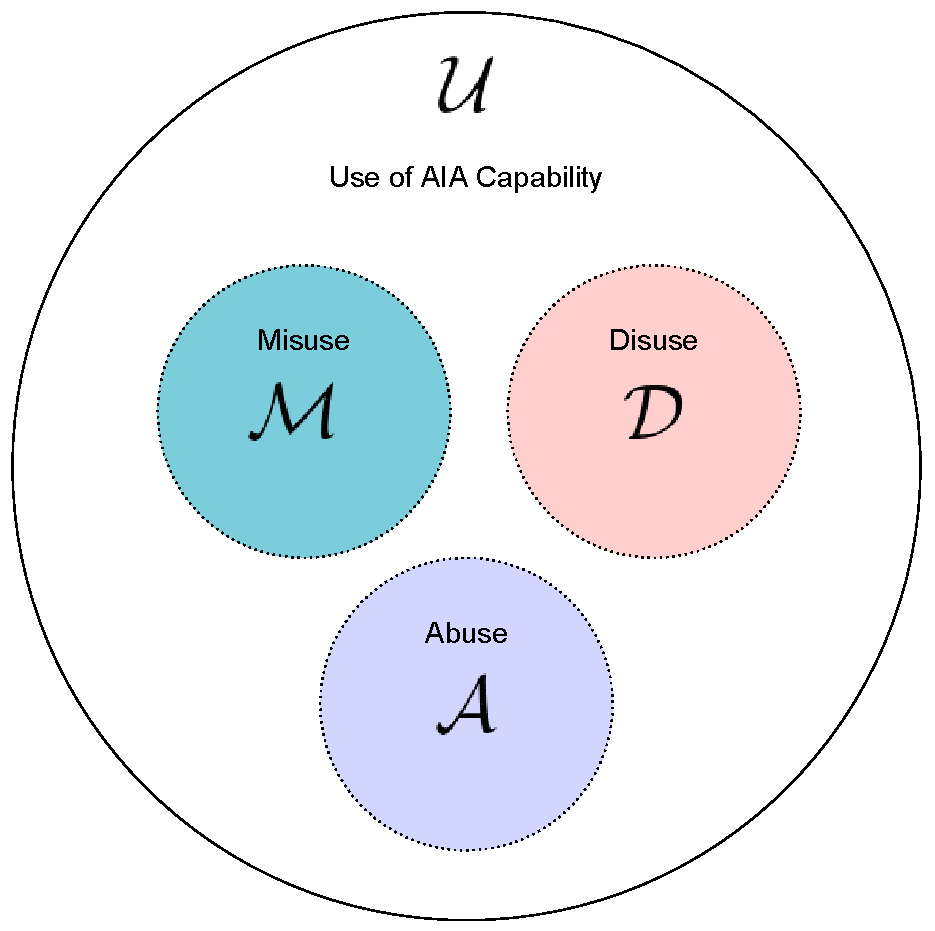
\includegraphics[width=0.6\textwidth]{Figures/misuse_disuse_abuse}
    	\caption{Graphic representing the total space of user actions, in which the inappropriate uses $\mathcal{M}$, $\mathcal{D}$, and $\mathcal{A}$ lie. The set of inappropriate uses $\mathcal{I}$ is the union of $\mathcal{M}$, $\mathcal{D}$, and $\mathcal{A}$. The appropriate set of actions $\mathcal{U}$ is the compliment of \mathcal{I}, or the part of $\mathcal{T}$ that does not include $\mathcal{I}$.}
    \end{figure}

\section{Different key points}
    \subsection{exemplar}
    \subsection{model based}
    \subsection{etc\ldots}

\section{Conclusion}
    Revisit the key ideas of the paper:

    \begin{itemize}
        \item trust is a key factor for human-agent interaction
        \item many fields care about it
        \item circumspection is a common framework
        \item circumspection has several key properties that encompass the different research fields
    \end{itemize}

\newpage
